
% TODO: appendix with Python

\chapter{Matrix multiplication}

So far, we've multiplied scalars by vectors
(p.~\pageref{scalarVectorMultiplication}), vectors by other vectors
(p.~\pageref{dotProduct}), scalars by matrices
(p.~\pageref{scalarMatrixMultiplication}), and even matrices by vectors
(p.~\pageref{matrixVectorMultiplication}). The only thing we haven't done yet
is multiply one entire matrix by another. That mysterious operation is the
subject of this chapter.

Luckily, we've already set ourselves up for success. As it will turn out,
matrix-matrix multiplication is really just matrix-\textit{vector}
multiplication ``in a loop''; \textit{i.e.}, repeated several times.

\section{When it's legal and what you get}

But let's not get ahead of ourselves. First, let's outline the very curious
rules for (1) when two matrices \textit{can} be multiplied at all (often they
can't), and (2) if they can, what the dimensions of the result are. These rules
will surprise you at first (they certainly did me).

Let's say we have two matrices called $A$ and $B$. Suppose that $A$ is an
$m\times n$ matrix ($m$ rows and $n$ columns), and that $B$ is a $p\times q$
matrix. Visually, here's what we've got:

\makeatletter
\newcommand\makebig[2]{%
  \@xp\newcommand\@xp*\csname#1\endcsname{\bBigg@{#2}}%
  \@xp\newcommand\@xp*\csname#1l\endcsname{\@xp\mathopen\csname#1\endcsname}%
  \@xp\newcommand\@xp*\csname#1r\endcsname{\@xp\mathclose\csname#1\endcsname}%
}
\makeatother

\makebig{Biggg} {3.5}
\makebig{Bigggg} {4.0}
\makebig{Biggggg} {4.5}

\vspace{-.15in}
\begin{align*}
m \Biggg\{
\overbrace{
\begin{bmatrix}
\smallblacksquare & \smallblacksquare & \cdots & \smallblacksquare \\
\smallblacksquare & \smallblacksquare & \cdots & \smallblacksquare \\
\vdots & \vdots & \cdots & \vdots \\
\smallblacksquare & \smallblacksquare & \cdots & \smallblacksquare \\
\end{bmatrix}}^n \ \  \smallblackcircle \ \ 
p \Biggg\{
\overbrace{
\begin{bmatrix}
\smallblacksquare & \smallblacksquare & \cdots & \smallblacksquare \\
\smallblacksquare & \smallblacksquare & \cdots & \smallblacksquare \\
\vdots & \vdots & \cdots & \vdots \\
\smallblacksquare & \smallblacksquare & \cdots & \smallblacksquare \\
\end{bmatrix}}^q
\ \ = \ \ \text{\LARGE ?}
\end{align*}
\vspace{-.15in}

\smallskip
Here are the rules:

\begin{center}
\begin{framed}
\begin{compactenum}
\label{matMultRules}
\item $n$ must be equal to $p$, or you can't multiply the matrices at all.
\item If $n$ does equal $p$, then you'll get an $m\times q$ matrix when you
multiply them.
\end{compactenum}
\end{framed}
\end{center}

Those rules are so strange and unexpected that it's worth taking a long moment
to stare at both the matrices and the rules and try to digest them.

\smallskip

Some concrete examples:

\begin{enumerate}
\itemsep.5em

\item Can we multiply a $3\times 2$ matrix by a $2\times 4$? Yes, since $n=2$
and $p=2$. And our result will be a $3\times 4$:

\vspace{-.15in}
\begin{align*}
3 \Biggg\{
\overbrace{
\begin{bmatrix}
\smallblacksquare & \smallblacksquare \\
\smallblacksquare & \smallblacksquare \\
\smallblacksquare & \smallblacksquare \\
\end{bmatrix}}^2 \ \  \cdot \ \ 
2 \Bigg\{
\overbrace{
\begin{bmatrix}
\smallblacksquare & \smallblacksquare & \smallblacksquare & \smallblacksquare \\
\smallblacksquare & \smallblacksquare & \smallblacksquare & \smallblacksquare \\
\end{bmatrix}}^4
\ \ = \ \ 
3 \Biggg\{
\overbrace{
\begin{bmatrix}
\smallblacksquare & \smallblacksquare & \smallblacksquare & \smallblacksquare \\
\smallblacksquare & \smallblacksquare & \smallblacksquare & \smallblacksquare \\
\smallblacksquare & \smallblacksquare & \smallblacksquare & \smallblacksquare \\
\smallblacksquare & \smallblacksquare & \smallblacksquare & \smallblacksquare \\
\end{bmatrix}}^4.
\end{align*}
\vspace{-.15in}

\item Can we multiply a $2\times 5$ matrix by a $5\times 3$? Yes, since $n=5$
and $p=5$. And we get a $2\times 3$:

\vspace{-.15in}
\begin{align*}
2 \Bigg\{
\overbrace{
\begin{bmatrix}
\smallblacksquare & \smallblacksquare& \smallblacksquare& \smallblacksquare& \smallblacksquare \\
\smallblacksquare & \smallblacksquare& \smallblacksquare& \smallblacksquare& \smallblacksquare \\
\end{bmatrix}}^5 \ \  \cdot \ \ 
5 \Biggggg\{
\overbrace{
\begin{bmatrix}
\smallblacksquare & \smallblacksquare & \smallblacksquare \\
\smallblacksquare & \smallblacksquare & \smallblacksquare \\
\smallblacksquare & \smallblacksquare & \smallblacksquare \\
\smallblacksquare & \smallblacksquare & \smallblacksquare \\
\smallblacksquare & \smallblacksquare & \smallblacksquare \\
\end{bmatrix}}^3
\ \ = \ \ 
2 \Bigg\{
\overbrace{
\begin{bmatrix}
\smallblacksquare & \smallblacksquare & \smallblacksquare \\
\smallblacksquare & \smallblacksquare & \smallblacksquare \\
\end{bmatrix}}^3.
\end{align*}
\vspace{-.15in}

\item Can we multiply a $4\times 3$ matrix by another $4\times 3$? No, since
$n=3$ but $p=4$. Sorry.

\vspace{-.15in}
\begin{align*}
4 \Bigggg\{
\overbrace{
\begin{bmatrix}
\smallblacksquare & \smallblacksquare & \smallblacksquare \\
\smallblacksquare & \smallblacksquare & \smallblacksquare \\
\smallblacksquare & \smallblacksquare & \smallblacksquare \\
\smallblacksquare & \smallblacksquare & \smallblacksquare \\
\end{bmatrix}}^3 \ \  \smallblackcircle \ \ 
4 \Bigggg\{
\overbrace{
\begin{bmatrix}
\smallblacksquare & \smallblacksquare & \smallblacksquare \\
\smallblacksquare & \smallblacksquare & \smallblacksquare \\
\smallblacksquare & \smallblacksquare & \smallblacksquare \\
\smallblacksquare & \smallblacksquare & \smallblacksquare \\
\end{bmatrix}}^3
\ \ = \ \ \text{NOPE}.
\end{align*}
\vspace{-.15in}
\end{enumerate}

It's sooo bizarre. Sometimes you multiply two biggish matrices together and get
a small one; sometimes you multiply narrow ones and get a tall one; sometimes
it seems like you'd get a valid answer and yet there is none.

Anyway, now that we have the ground rules for what the resulting matrix will be
shaped like (if there even is one) let's talk about actually calculating the
entries. I'm going to give you \textit{three} different ways to think about
this, each of which sheds a different light on the operation.

\section{Way \#1: Lather, rinse, repeat}

\index{matrix-vector multiplication}

The first way is to view the matrix multiplication $A \cdot B$ as
\textbf{repeated matrix-vector multiplication}, where the matrix is $A$ and the
vectors are the \textbf{columns} of $B$. The final answer is formed by
stitching together the results of the individual matrix-vector multiplications.

Let's see it in action. If you remember the procedure on
p.~\pageref{matrixVectorMultiplication}, you can confirm that if we perform
this matrix-vector multiplication:

\vspace{-.15in}
\begin{align*}
\begin{bmatrix}
2 & 1 & 5 \\
0 & 3 & -2 \\
\end{bmatrix} \cdot
\begin{bmatrix}
0 \\ 0 \\ 7 \\
\end{bmatrix},
\end{align*}
\vspace{-.15in}

we'll get the answer

\vspace{-.15in}
\begin{align*}
\begin{bmatrix}
35 \\ -14 \\
\end{bmatrix}.
\end{align*}
\vspace{-.15in}

\smallskip
And if we do this:

\vspace{-.15in}
\begin{align*}
\begin{bmatrix}
2 & 1 & 5 \\
0 & 3 & -2 \\
\end{bmatrix} \cdot
\begin{bmatrix}
9 \\ 99 \\ 999 \\
\end{bmatrix},
\end{align*}
\vspace{-.15in}

we'll get this:

\vspace{-.15in}
\begin{align*}
\begin{bmatrix}
5112 \\ -1701 \\
\end{bmatrix}.
\end{align*}
\vspace{-.15in}

\smallskip
Finally, if we do this:

\vspace{-.15in}
\begin{align*}
\begin{bmatrix}
2 & 1 & 5 \\
0 & 3 & -2 \\
\end{bmatrix} \cdot
\begin{bmatrix}
-13 \\ -13 \\ -13 \\
\end{bmatrix},
\end{align*}
\vspace{-.15in}

we'll get this:

\vspace{-.15in}
\begin{align*}
\begin{bmatrix}
-104 \\ -13 \\
\end{bmatrix}.
\end{align*}
\vspace{-.15in}

\smallskip

Notice what I did there. I took the \textit{same} $2\times 3$ matrix each time,
and multiplied it by some vector -- a weird one, to help jog your memory in a
moment -- to get an answer.

All right. Now let's see what happens if I perform the following
matrix-\textit{matrix} multiplication:

\vspace{-.15in}
\begin{align*}
\begin{bmatrix}
2 & 1 & 5 \\
0 & 3 & -2 \\
\end{bmatrix} \cdot
\begin{bmatrix}
0 & 9 & -13 \\
0 & 99 & -13 \\
7 & 999 & -13 \\
\end{bmatrix} \ = \ {\LARGE ?}
\end{align*}
\vspace{-.15in}

Examine the columns of the right-hand matrix: they should ring a bell. Each
\textit{column} is one of the \textit{vectors} that we just multiplied our
matrix by to get a columnar answer. The result of this operation is achieved by
simply putting all those columnar answers together:

\vspace{-.15in}
\begin{align*}
\begin{bmatrix}
2 & 1 & 5 \\
0 & 3 & -2 \\
\end{bmatrix} \cdot
\begin{bmatrix}
0 & 9 & -13 \\
0 & 99 & -13 \\
7 & 999 & -13 \\
\end{bmatrix} =
\begin{bmatrix}
35 & 5112 & -104 \\
-14 & -1701 & -13 \\
\end{bmatrix}.
\end{align*}
\vspace{-.15in}

\index{Bond, James}

See how that works? The result of the multiplication is just the three
individual matrix-vector products, all concatenated together in an ``answer
matrix.'' The left column of our answer is ${\scriptsize \begin{bmatrix} 35 \\
-14 \\ \end{bmatrix}}$, which is exactly what we got when we multiplied that
left-hand matrix by James Bond. The right column of our answer is ${\scriptsize
\begin{bmatrix} -104 \\ -13 \\ \end{bmatrix}}$, which is what we got when we
multiplied the matrix by triple $-13$'s. And the middle column of the answer is
the matrix times the stack of nines. So you can see that matrix-\textit{matrix}
multiplication is really just repeated matrix-\textit{vector} multiplication.

This way of thinking about matrix multiplication might be the one that
resonates most strongly with you. (It did for me.)

\section{Way \#2: All possible dot products}

On the other hand, maybe you'll like this one better. Matrix-matrix
multiplication can also be viewed as \textbf{all possible dot products} between
the \textbf{rows} of $A$ and the \textbf{columns} of $B$.

Flash back for a moment to \textit{A Cool, Brisk Walk} chapter 6, and the
Fundamental Theorem of Counting. Answer this question: ``You have two choices
of appetizer, and three choices of entr\'{e}e. How many different dinner
combinations are possible?''

The answer is six, since each of the two appetizers can go with any of the
three entr\'{e}es. So you could choose:

\begin{compactenum}
\item shrimp cocktail, filet mignon
\item shrimp cocktail, chicken pesto
\item shrimp cocktail, eggplant parmigiana
\item artichoke dip, filet mignon
\item artichoke dip, chicken pesto
\item artichoke dip, eggplant parmigiana
\end{compactenum}

Now back to matrices. If I multiply these two matrices together:

\vspace{-.15in}
\begin{align*}
\begin{bmatrix}
2 & 1 & 5 \\
0 & 3 & -2 \\
\end{bmatrix} \ \text{and} \ 
\begin{bmatrix}
0 & 9 & -13 \\
0 & 99 & -13 \\
7 & 999 & -13 \\
\end{bmatrix},
\end{align*}
\vspace{-.15in}

how many possible dot products are there between \textit{rows} of $A$ and
\textit{columns} of $B$?

The answer is six, since each of the two $A$ rows can go with any of the three
$B$ rows. The possibilities are:

\begin{compactenum}
\item $[\ 2\ \ 1\ \ 5\ ]$ and $[\ 0\ \ 0\ \ 7\ ]$
\item $[\ 2\ \ 1\ \ 5\ ]$ and $[\ 9\ \ 99\ \ 999\ ]$
\item $[\ 2\ \ 1\ \ 5\ ]$ and $[\ -13\ \ -13\ \ -13\ ]$
\item $[\ 0\ \ 3\ \ -2\ ]$ and $[\ 0\ \ 0\ \ 7\ ]$
\item $[\ 0\ \ 3\ \ -2\ ]$ and $[\ 9\ \ 99\ \ 999\ ]$
\item $[\ 0\ \ 3\ \ -2\ ]$ and $[\ -13\ \ -13\ \ -13\ ]$
\end{compactenum}

(Note \textit{very} carefully that we use the \textit{columns} of $B$, not the
rows!)

\smallskip
Very well. Let's compute all those dot products then:

\begin{compactitem}
\item $[\ 2\ \ 1\ \ 5\ ] \cdot [\ 0\ \ 0\ \ 7\ ] = 35$
\item $[\ 2\ \ 1\ \ 5\ ] \cdot [\ 9\ \ 99\ \ 999\ ] = 5112$
\item $[\ 2\ \ 1\ \ 5\ ] \cdot [\ -13\ \ -13\ \ -13\ ] = -104$
\item $[\ 0\ \ 3\ \ -2\ ] \cdot [\ 0\ \ 0\ \ 7\ ] = -14$
\item $[\ 0\ \ 3\ \ -2\ ] \cdot [\ 9\ \ 99\ \ 999\ ] = -1701$
\item $[\ 0\ \ 3\ \ -2\ ] \cdot [\ -13\ \ -13\ \ -13\ ] = -13$
\end{compactitem}

\smallskip
Those six dot products are precisely the entries in our answer matrix:

\vspace{-.15in}
\begin{align*}
\begin{bmatrix}
35 & 5112 & -104 \\
-14 & -1701 & -13 \\
\end{bmatrix}.
\end{align*}
\vspace{-.15in}

The only thing you have to be careful of is which answer goes in which place.
The rule is:

\begin{framed}
The dot product of row $i$ of $A$ and column $j$ of $B$ goes in
row $i$, column $j$ of the answer.
\end{framed}

A sensible arrangement, I think you'll agree. Multiplying row 0 with column 0
will give us the entry in row 0, column 0 of our answer. Multiplying row 14
with column 9 will give us the entry in row 14, column 9 of our answer. And so
forth.

In terms of our current example, the reason that the number 5112 goes in the
\textit{top middle} of our answer (as opposed to the bottom left, or anywhere
else) is that 5112 is the dot product of the \textit{top} row of $A$ ($[\ 2\ \
1\ \ 5\ ]$) with the \textit{middle} column of $B$ ($[\ 9\ \ 99\ \ 999\ ]$).
Be sure to practice with this so you don't get numbers out of place.

\smallskip

\index{matchmaker@\texttt{matchmaker.com}}

It might help to keep in mind possible applications here. Why would we ever
want to compute ``all possible dot products?'' Well, think back to our
matchmaker example. Let's say we have 4 women and 5 men, each of whom has
completed a survey. Finding all the compatibilities -- \textit{i.e.},
predicting the dating success of all possible pairings -- is precisely
computing the dot product of every gal with every guy (assuming
heterosexuality). That's 20 possible dot products, which we can calculate with
a single matrix multiplication.

% TODO: explain that we need "Women times TRANSPOSE of men" not "women times
% men."

\section{Way \#3: Several linear combinations}

Our third and final way to think about matrix multiplication is in terms of
linear combinations. Remember (from p.~\pageref{linearComboOfColumns}) that
every matrix-\textit{vector} multiplication $A \cdot
\overrightarrow{\textbf{x}}$ is essentially specifying some linear combination
of $A$'s \textit{columns}. If we multiply $A$ by the vector ${\scriptsize
\begin{bmatrix} 3 \\ 5 \\ \end{bmatrix}}$, we're saying ``I'd like 3 copies of
$A$'s first column, plus 5 copies of its second column, please.''

Matrix multiplication is simply asking for several \textit{different} linear
combinations. If we multiply a matrix $A$ by this one:

\vspace{-.15in}
\begin{align*}
\begin{bmatrix}
0 & 9 & -13 \\
0 & 99 & -13 \\
7 & 999 & -13 \\
\end{bmatrix},
\end{align*}
\vspace{-.15in}

we're requesting the following:

\begin{quote}
\index{credit card}
\textit{
``Hello, I'd like to put in an order for three things. First, I'd like 7 copies
of $A$'s third column (ignore the first two). Additionally, I'd like 9 copies
of its first column, 99 copies of its second column, and 999 copies of its
third column, all added together. Finally, please give me $-13$ copies of each
of its columns, again added together. Thanks! You should have my credit card
number on file.''
}
\end{quote}

To fulfill this order, we compute each of the three linear combinations
requested. Using the same $A$ matrix we've been using (${\scriptsize
\begin{bmatrix} 2 & 1 & 5 \\ 0 & 3 & -2 \end{bmatrix}}$) this amounts to:

\vspace{-.15in}
\begin{align*}
\text{First combination: } &7
\begin{bmatrix}
5 \\
-2 \\
\end{bmatrix} =
\begin{bmatrix}
35 \\
-14 \\
\end{bmatrix} \\
\text{Second combination: } &9
\begin{bmatrix}
2 \\
0 \\
\end{bmatrix} + 99
\begin{bmatrix}
1 \\
3 \\
\end{bmatrix} + 999
\begin{bmatrix}
5 \\
-2 \\
\end{bmatrix} =
\begin{bmatrix}
5112 \\
-1701 \\
\end{bmatrix} \\
\text{Third combination: } &-13
\begin{bmatrix}
2 \\
0 \\
\end{bmatrix} -13
\begin{bmatrix}
1 \\
3 \\
\end{bmatrix} -13
\begin{bmatrix}
5 \\
-2 \\
\end{bmatrix} =
\begin{bmatrix}
-104 \\
-13 \\
\end{bmatrix}
\end{align*}
\vspace{-.15in}

Packaging up all those results again gives us:

\vspace{-.15in}
\begin{align*}
\begin{bmatrix}
35 & 5112 & -104 \\
-14 & -1701 & -13 \\
\end{bmatrix}.
\end{align*}
\vspace{-.15in}

Same answer no matter which of the three ways we think about it.

\section{Outer and inner products}

All right. Now for some surprises.

\index{row vector}
\index{column vector}

Remember (p.~\pageref{rowAndColVectors}) that we will sometimes want to treat a
vector as a sort of degenerate matrix: a matrix with only one row, or only one
column. And we will sometimes want to do this matrix multiplication thing with
two vectors, treating one of them as a row vector and the other as a column
vector. Which one is which makes a tremendous difference.

As an illustration, I'm going to define vectors $\overrightarrow{\textbf{x}}$
and $\overrightarrow{\textbf{y}}$ this way:

\vspace{-.15in}
\begin{align*}
\overrightarrow{\textbf{x}} =
\begin{bmatrix}
3 & 1 & 2 \\
\end{bmatrix}, \quad 
\overrightarrow{\textbf{y}} =
\begin{bmatrix}
5 \\  4 \\ -3 \\
\end{bmatrix}.
\end{align*}
\vspace{-.15in}

So $\overrightarrow{\textbf{x}}$ is a row vector, and
$\overrightarrow{\textbf{y}}$ is a column vector. Put another way,
$\overrightarrow{\textbf{x}}$ can be thought of as a $1\times 3$ matrix, and
$\overrightarrow{\textbf{y}}$ as a $3\times 1$ matrix.

Now if we do treat these as matrices, then performing the operation
$\overrightarrow{\textbf{x}} \cdot \overrightarrow{\textbf{y}}$ gives us:

\vspace{-.15in}
\begin{align*}
\overrightarrow{\textbf{x}} \cdot \overrightarrow{\textbf{y}} =
\begin{bmatrix}
3 & 1 & 2 \\
\end{bmatrix} \cdot
\begin{bmatrix}
5 \\ 4 \\ -3 \\
\end{bmatrix} = 13.
\end{align*}
\vspace{-.15in}

It's just the dot product, of course, calculated in the usual way.

Now suppose I swap the order, and compute $\overrightarrow{\textbf{y}}$ times
$\overrightarrow{\textbf{x}}$ instead. What would I get? The answer will surely
surprise you:

\vspace{-.15in}
\begin{align*}
\overrightarrow{\textbf{y}} \cdot \overrightarrow{\textbf{x}} =
\begin{bmatrix}
5 \\ 4 \\ -3 \\
\end{bmatrix} \cdot
\begin{bmatrix}
3 & 1 & 2 \\
\end{bmatrix} =
\begin{bmatrix}
15 & 5 & 10 \\
12 & 4 & 8 \\
-9 & -3 & -6 \\
\end{bmatrix}.
\end{align*}
\vspace{-.15in}

Hooooooo...wut?! $\overrightarrow{\textbf{x}}$ times
$\overrightarrow{\textbf{y}}$ is the \textit{number} 13, but
$\overrightarrow{\textbf{y}}$ times $\overrightarrow{\textbf{x}}$ is an entire
\textit{grid} full of numbers?

Yes it is. Here's why. 

Remember our rules from p.~\pageref{matMultRules}. First, we can only multiply
two matrices if $n=p$. And that's true here whether we do
$\overrightarrow{\textbf{x}} \cdot \overrightarrow{\textbf{y}}$ or
$\overrightarrow{\textbf{y}} \cdot \overrightarrow{\textbf{x}}$. But the second
rule tells us that the answer will be a $m\times q$ matrix. If we put
$\overrightarrow{\textbf{x}}$ on the left, then $\overrightarrow{\textbf{x}}
\cdot \overrightarrow{\textbf{y}}$ will give us a $1\times 1$ matrix. But if we
put $\overrightarrow{\textbf{y}}$ on the left, then
$\overrightarrow{\textbf{y}} \cdot \overrightarrow{\textbf{x}}$ must give us a
$3\times 3$ matrix. Strange but true.

\index{inner product}
\index{outer product}

Btw, when we do the first thing -- treat the vector on the left-hand side of
the multiplication as a row vector, and the other as a column vector -- it's
called the \textbf{inner product} of the two vectors. The other way is called
the \textbf{outer product}.

\section{$A\cdot A^\intercal$ vs.~$A^\intercal \cdot A$} 

\index{transpose}

Here's another interesting consequence of our operation. As we've seen, you
certainly can't multiply a matrix $A$ by just ``any old thing,'' since rule 1
on p.~\pageref{matMultRules} says that $n$ must equal $p$.

You can, however, \textit{always} perform the operation $A\cdot A^\intercal$,
no matter what dimensions $A$ is. That's because if $A$ is, say, $17\times 28$,
then $A^\intercal$ will be $28\times 17$, and $n=p$ (both are 28) as required.
You'll get a $17\times 17$ matrix if you do that.

You also can \textit{always} perform the operation $A^\intercal \cdot A$.
Again, if $A$ is $17\times 28$, then $A^\intercal$ will be $28\times 17$, and
so again $n=p$ (both are 17). You'll get a $28\times 28$ matrix if you do that.

Here's an example, smaller so it fits on the page. Let's say $A$ is

\vspace{-.15in}
\begin{align*}
\begin{bmatrix}
2 & 20 & 3 & -2 & -4 \\
-5 & 1 & 4 & 1 & 9 \\
\end{bmatrix}.
\end{align*}
\vspace{-.15in}

The two operations give us:

\vspace{-.15in}
\begin{align*}
A\cdot A^\intercal = 
\begin{bmatrix}
2 & 20 & 3 & -2 & -4 \\
-5 & 1 & 4 & 1 & 9 \\
\end{bmatrix} \cdot
\begin{bmatrix}
2 & -5 \\
20 & 1 \\
3 & 4 \\
-2 & 1 \\
-4 & 9 \\
\end{bmatrix}  =
\begin{bmatrix}
433 & -16 \\
-16 & 124 \\
\end{bmatrix},
\end{align*}
\vspace{-.15in}

and 

\vspace{-.15in}
\begin{align*}
A^\intercal \cdot A = 
\begin{bmatrix}
2 & -5 \\
20 & 1 \\
3 & 4 \\
-2 & 1 \\
-4 & 9 \\
\end{bmatrix} \cdot
\begin{bmatrix}
2 & 20 & 3 & -2 & -4 \\
-5 & 1 & 4 & 1 & 9 \\
\end{bmatrix} = \\
\begin{bmatrix}
29 & 35 & -14 & -9 & -53 \\
35 & 401 & 64 & -39 & -71 \\
-14 & 64 & 25 & -2 & 24 \\
-9 & -39 & -2 & 5 & 17 \\
-53 & -71 & 24 & 17 & 97 \\
\end{bmatrix}.
\end{align*}
\vspace{-.15in}

\index{symmetric matrix}

Two other intriguing facts are worth noting here, one of which you may have
noticed. If you run your eyeballs carefully over those two results, you'll see
that both of them are \textbf{symmetric matrices}. This is always true of a
matrix times its transpose, and that turns out to be important for some
applications.

The other fact -- certainly not ascertainable to my eyeballs, at least -- is
that both of these matrices have only \textit{rank 2}. That's not surprising
about $A\cdot A^\intercal$, since it's just a $2\times 2$ anyway. But it is
very surprising about $A^\intercal \cdot A$. That's a $5\times 5$ matrix with
only \textit{two} linearly independent columns!

And this is always true. When you multiply a matrix by its transpose, either
way you do it, the rank will only be the \textit{lower} of the two dimensions.

The way I think of it is this. When you take a tall matrix (like our $5\times
2$, above) and multiply it by a wide one (the $2\times 5$), yes you're going to
get a result with large dimensions. Sure. But in a way, you only put ``two
columns' worth'' of information into the operation. The result is a large
$5\times 5$, but that's misleading, because there just isn't enough information
present in those 25 entries to represent five independent directions. The
$5\times 5$ result is brittle, containing only two columns' worth of
information spread out over a large landscape. It's almost as if I wrote a
fourteen-sentence paragraph with only three sentences repeated again and again,
with the words rescrambled a bit each time. Sure, it looks like a long
paragraph at first glance, but try reading it and you'll recognize how little
information it really contains.

\section{Associative, but not commutative}

\label{associative}

\index{commutative}
\index{associative (operation)}

The next surprising thing I'll point out is that matrix multiplication does
\textit{not} follow one of the laws of plain-Jane multiplication that you're
used to counting on. Namely, matrix multiplication is \textit{not} commutative.

You're so accustomed to this being true that it's positively jarring. Ever
since Mrs.~Jones taught you in second grade, you've safely relied on the fact
that:

\vspace{-.15in}
\begin{align*}
115 \cdot 272 = 272 \cdot 115.
\end{align*}
\vspace{-.15in}

It might be a pain to work out the answer, but at least you've know without
even thinking that it doesn't matter which order you do the multiplication in.

But \textit{oh!}~this totally does not work with matrix multiplication. Taking
two matrices at random:

\vspace{-.15in}
\begin{align*}
A =
\begin{bmatrix}
4 & 2 \\
2 & 3 \\
\end{bmatrix},
B =
\begin{bmatrix}
1 & -1 \\
2 & 0 \\
\end{bmatrix}\\
\end{align*}
\vspace{-.55in}
\begin{align*}
A \cdot B &=
\begin{bmatrix}
8 & -4 \\
8 & -2 \\
\end{bmatrix}, \\
B \cdot A &=
\begin{bmatrix}
2 & -1 \\
8 & 4 \\
\end{bmatrix}\ {\footnotesize \textit{surprise!}}
\end{align*}
\vspace{-.15in}

Not even close to the same thing. And in general, matters are even worse
because you normally can't even \textit{do} the operation both ways! (If $A$
were a $2\times 4$, for example, and $B$ a $4\times 3$, then $A \cdot B$ would
give you a $2\times 3$ matrix but $B \cdot A$ is impossible.) You actually have
to really work at it to come up with two matrices whose product is the same
both ways.

Nothing much to say here except to stay on your toes.

Another ``given,'' however, \textit{is} true of matrices, and a good thing,
too. That's the \textbf{associative} property. This means that if you're
multiplying together a string of matrices, it doesn't matter which
multiplication you perform first. In other words, for any three matrices $A$,
$B$, and $C$:

\vspace{-.15in}
\begin{align*}
(A \cdot B) \cdot C =
A \cdot (B \cdot C).
\end{align*}
\vspace{-.15in}

Again, an example to illustrate:

\vspace{-.15in}
\begin{align*}
A =
\begin{bmatrix}
4 & 2 \\
2 & 3 \\
\end{bmatrix},
B =
\begin{bmatrix}
1 & -1 \\
2 & 0 \\
\end{bmatrix},
C =
\begin{bmatrix}
3 & 4 \\
1 & 5 \\
\end{bmatrix}\\
\end{align*}
\vspace{-.55in}
\begin{align*}
(A \cdot B) \cdot C =
\begin{bmatrix}
8 & -4 \\
8 & -2 \\
\end{bmatrix} \cdot
\begin{bmatrix}
3 & 4 \\
1 & 5 \\
\end{bmatrix} &=
\begin{bmatrix}
20 & 12 \\
22 & 22 \\
\end{bmatrix}, \\
A \cdot (B \cdot C) =
\begin{bmatrix}
4 & 2 \\
2 & 3 \\
\end{bmatrix} \cdot
\begin{bmatrix}
2 & -1 \\
6 & 8 \\
\end{bmatrix} &=
\begin{bmatrix}
20 & 12 \\
22 & 22 \\
\end{bmatrix}. \quad \checkmark
\end{align*}
\vspace{-.15in}

\index{Cartesian plane}

And this always works.

One reason this is nice has to do with linear operators. Recall from
section~\ref{linearOps} (pp.~\pageref{linearOps}--\pageref{endLinearOps}) that
we can create operators to scale, flip, and rotate points in the Cartesian
plane. To review:

\vspace{-.15in}
\begin{align*}
\begin{bmatrix}
2 & 0 \\
0 & 2 \\
\end{bmatrix}
\quad & \text{stretch points twice as far from the origin}\\
\begin{bmatrix}
.866 & -.5 \\
.5 & .866 \\
\end{bmatrix}
\quad & \text{rotate points 30\degree\ counterclockwise}\\
\begin{bmatrix}
-1 & 0 \\
0 & 1 \\
\end{bmatrix}
\quad & \text{flip points horizontally across the $y$-axis}\\
\end{align*}
\vspace{-.15in}

Multiplying any of these matrices by a vector has the desired effect.

\medskip

Now suppose we wanted to perform \textit{several} of these operations on a
vector. For example, take a random point $(8.5, 19)$. To stretch, rotate,
\textit{and} flip it, we'd do this:

\vspace{-.15in}
\begin{align*}
\begin{bmatrix}
2 & 0 \\
0 & 2 \\
\end{bmatrix} \cdot
\begin{bmatrix}
.866 & -.5 \\
.5 & .866 \\
\end{bmatrix} \cdot
\begin{bmatrix}
-1 & 0 \\
0 & 1 \\
\end{bmatrix} \cdot
\begin{bmatrix}
8.5 \\
19 \\
\end{bmatrix}.
\end{align*}
\vspace{-.15in}

This works out to ${\scriptsize \begin{bmatrix} -33.722 \\ 24.408 \\
\end{bmatrix}}$ if you're keeping score at home.

\index{Bowser}

Now often instead of transforming a single point, we want to transform an
entire image, which contains multiple points. Imagine calculating every pixel
of Bowser as his Kart trips over a green shell and spins towards the side of
the screen. We can take advantage of the associativity of matrix multiplication
to pre-compute a \textit{single} matrix that will
stretch/flip/rotate/squish/whatever any point we care to multiply it by:

\vspace{-.15in}
\begin{align*}
T = 
\begin{bmatrix}
2 & 0 \\
0 & 2 \\
\end{bmatrix} \cdot
\begin{bmatrix}
.866 & -.5 \\
.5 & .866 \\
\end{bmatrix} \cdot
\begin{bmatrix}
-1 & 0 \\
0 & 1 \\
\end{bmatrix} =
\begin{bmatrix}
-1.732 & -1 \\
-1 & 1.732 \\
\end{bmatrix}.
\end{align*}
\vspace{-.15in}

This makes our game engine run a lot faster, since we don't have to do all
those calculations separately for every point in the image. Instead, we
calculate our $T$ matrix (for \textbf{t}ransformation) just once, and then
multiply it by every point.

In fact, if we have all of Bowser's pixels in a $2\times 1000$ matrix:

\vspace{-.15in}
\begin{align*}
B =
\begin{bmatrix}
18 & 19 & 22 & 32 & 34 & \cdots & 195 \\
9 & 9 & 11 & 14 & 19 & \cdots & 212 \\
\end{bmatrix},
\end{align*}
\vspace{-.15in}

then we can compute what pixels to draw in the next frame with just one
operation: $T \cdot B$!

\vspace{-.15in}
\begin{align*}
B_{\text{next}} = T \cdot B =
\begin{bmatrix}
-1.732 & -1 \\
-1 & 1.732 \\
\end{bmatrix} \cdot
\begin{bmatrix}
18 & 19 & 22 & 32 & 34 & \cdots & 195 \\
9 & 9 & 11 & 14 & 19 & \cdots & 212 \\
\end{bmatrix}.
\end{align*}
\vspace{-.15in}

You gotta admit, that's pretty neat.

% TODO: multiplying two symmetric matrices together does not normally give a
% symmetric matrix! (Wut?!)  Important for social network analysis.

\pagebreak

\section{The ``identity'' matrix}

\label{identityMatrixExplanation}
\index{identity matrix}
\index{diagonal, of a matrix}

Remember back on p.~\pageref{identityMatrix} how we defined ``identity
matrices?'' They looked like this:

\vspace{-.15in}
\begin{align*}
\begin{bmatrix}
1 & 0 & 0 \\
0 & 1 & 0 \\
0 & 0 & 1 \\
\end{bmatrix}
\end{align*}
\vspace{-.15in}

They could be any size, but they were always square, and they always had 1's on
the diagonal and 0's everywhere else.

I promised to tell you why this kind of matrix was called an ``identity''
matrix, and now's the time. It's simply because when you multiply it by any
matrix, you get that same matrix back. Let's try it:

\vspace{-.15in}
\begin{align*}
\begin{bmatrix}
1 & 0 & 0 \\
0 & 1 & 0 \\
0 & 0 & 1 \\
\end{bmatrix} \cdot
\begin{bmatrix}
7 & 7 & 9 & 4 \\
-10 & -5 & 5 & 3 \\
17 & 16 & 14 & 13 \\
\end{bmatrix} =
\begin{bmatrix}
7 & 7 & 9 & 4 \\
-10 & -5 & 5 & 3 \\
17 & 16 & 14 & 13 \\
\end{bmatrix}.
\end{align*}
\vspace{-.15in}

Yep, it works. And you can put the identity matrix on either the left side or
the right of the multiplication, and it still works.

\index{identity element}

Because of this property, the identity matrix plays the same role as the number
zero in addition (0 plus any number is that same number) and the number one in
multiplication (1 times any number is that same number). Those numbers are
called the ``identity elements'' for those operations, since you get the
``identical'' number back when you use them. Same reasoning here.

\section{The ``inverse'' of a matrix}

\label{matrixInverse}
\index{reciprocal}

In high school (or maybe middle school) you learned what the
\textbf{reciprocal} of a number was: namely, the number that you had to
multiply it by to get 1. So the reciprocal of $3$ was $\frac{1}{3}$, since $3
\cdot \frac{1}{3} = 1$. Similarly, the reciprocal of $-\frac{1}{5}$ was $-5$
and the reciprocal of $-\frac{\pi}{8}$ was $-\frac{8}{\pi}$. Easy.

\index{inverse}
\index{identity element}
\index{additive inverse}
\index{multiplicative inverse}

Another name for the reciprocal of a number, by the way, is the
``multiplicative \textbf{inverse}.'' If you want to ``invert'' the number $3$,
you use $\frac{1}{3}$; this sends $3$ back to 1, which the identity element for
multiplication. (Similarly, the ``\textit{additive} inverse'' of $3$ is $-3$,
since if you're \textit{adding} instead of multiplying, that's the number you
use to send $3$ back to 0, which is the identity element for addition.)

\smallskip

Now how do you think this concept would apply to \textit{matrix}
multiplication? I give you a square matrix $A$, and I ask you to find its
``reciprocal'' -- that is, its \textbf{inverse}. The answer I'm looking for is
\textit{the matrix you'd multiply by $A$ to get the identity matrix.} Ooo,
deep.

Now there are many differently-sized identity matrices, but you can probably
guess that I'm referring to the one of the same dimensions as $A$. In other
words, if I give you:

\vspace{-.15in}
\begin{align*}
A = 
\begin{bmatrix}
5 & 6 & 7 \\
2 & 1 & 2 \\
9 & 8 & -2 \\
\end{bmatrix},
\end{align*}
\vspace{-.15in}

I'm asking for the matrix that we can multiply by $A$ and get:

\vspace{-.15in}
\begin{align*}
\begin{bmatrix}
1 & 0 & 0 \\
0 & 1 & 0 \\
0 & 0 & 1 \\
\end{bmatrix},
\end{align*}
\vspace{-.15in}

since that one's the right size.

\smallskip
Incidentally, the notation we use for $A$'s inverse is not $\frac{1}{A}$, as
you might expect, but $A^{-1}$. It's pronounced ``$A$ inverse.''
\smallskip

Now it's not at all obvious that (1) there even \textit{is} an inverse matrix
for $A$, nor that (2) there's only \textit{one} inverse matrix for $A$. And in
fact we'll see in the next section that sometimes there is no inverse for a
matrix $A$ (although there's never more than one, as it happens). But usually
there is exactly one, as it turns out. And that will be good news.

Why good news? Why do we care?

\subsection{Simultaneous equations}

There are several important reasons why we care, as it happens. In this section
I'm going to talk about only one of them, and it'll seem at first as if I've
veered off-topic into something that has nothing to do with linear algebra at
all. But stay with me.

\index{simultaneous equations}

From your pre-college days, you undoubtedly remember solving
\textbf{simultaneous equations}. For example, faced with this:

\vspace{-.25in}
\begin{align*}
2x - 3y &= 1 \\
3x + y &= 7,
\end{align*}
\vspace{-.25in}

\label{hellaciousAlgebra}

you could use a variety of different techniques to work out that $x=2$ and
$y=1$. For me, the least hateful way of solving those problems was to use
substitution: get one variable in terms of the other (like fiddling with that
first equation to get $x = \frac{1+3y}{2}$, then plugging $\frac{1+3y}{2}$ in
for $x$ in the second equation). But you may have done the thing where you
multiply one of the entire equations by some number and add it to the other
one, or maybe you learned yet another way. As long as you don't screw up any of
your math, you'll get the same answer regardless of technique.

The reason these are called ``simultaneous equations,'' by the way, is that
you're looking for values of $x$ and $y$ that \textit{simultaneously} make both
equations true. It's easy to just eyeball it and find an $x$ and a $y$ that
make just one of the equations true. But getting values that satisfy both
equations simultaneously is the trick.

\smallskip

You may have done more than just ``two equations, two unknowns'' in high
school, like this problem that has three of each:

\vspace{-.25in}
\begin{align*}
6x + 2y - 4z &= -4 \\
x + y + 2z &= 8 \\
2x - 2y + 8z &= 4.
\end{align*}
\vspace{-.25in}

(*Shudder*) With enough laborious steps, and enough caffeine, you'll manage to
crank out the correct answer which is $x=-1$, $y=5$, $z=2$.

It probably won't surprise you to learn that it's also possible to solve five
equations in five unknowns, or a hundred equations in a hundred unknowns,
\textit{etc.} It may surprise you to learn that there are situations where we
actually need to \textit{do} that, because the equations stand for real
relationships between real quantities and solving simultaneous equations is how
we figure out the real values.

Luckily for the human race, all that error-prone algebraic manipulation
required to solve a hundred simultaneous equations this way (or even a few
thousand) is utterly unnecessary. Matrices come brilliantly to our rescue.

Let me recast the first problem above,

\vspace{-.25in}
\begin{align}
\label{ordEq1}
2x - 3y &= 1 \\
\label{ordEq2}
3x + y &= 7,
\end{align}
\vspace{-.25in}

in the following way:

\vspace{-.15in}
\begin{align}
\label{matEq}
\begin{bmatrix}
2 & -3 \\
3 & 1 \\
\end{bmatrix} \cdot
\begin{bmatrix}
x \\ y \\
\end{bmatrix} =
\begin{bmatrix}
1 \\ 7 \\
\end{bmatrix}.
\end{align}
\vspace{-.15in}

Whoa. Sudden leap from high school back to college. But do you see the
connection? Stare hard at the matrices in equation \ref{matEq} and compare them
with the original equations \ref{ordEq1} and \ref{ordEq2}. You'll realize that
the matrix entries are the \textit{coefficients} of the equations, and the
right-most vector has the values from the equations' right-hand-sides.

\index{matrix-vector multiplication}

A light bulb will go on for you as soon as you realize that the matrix equation
is \textit{exactly the same} as the two ordinary equations! That's because when
we do matrix-vector multiplication, we do two separate things: (1) take the dot
product of the top matrix row and the ${\scriptsize \begin{bmatrix} x \\ y
\end{bmatrix}}$ vector, and (2) take the dot product of the \textit{bottom}
matrix row and the ${\scriptsize \begin{bmatrix} x \\ y \end{bmatrix}}$ vector.
When we do this, we get:

\vspace{-.15in}
\begin{align*}
\begin{bmatrix}
2x - 3y \\
3x + 1 \\
\end{bmatrix} =
\begin{bmatrix}
1 \\ 7 \\
\end{bmatrix}.
\end{align*}
\vspace{-.15in}

This is just another way of saying \textit{exactly} the same thing that
\ref{ordEq1} and \ref{ordEq2} do.

\smallskip

Okay, so why is this important? Here's why. Suppose we could find the
\textit{inverse} of the left matrix in equation \ref{matEq}. We'll call it
$A^{-1}$. Now if we multiply both sides of that equation by $A^{-1}$ we'd get:

\vspace{-.15in}
\begin{align*}
A^{-1} \cdot
\begin{bmatrix}
2 & -3 \\
3 & 1 \\
\end{bmatrix} \cdot
\begin{bmatrix}
x \\ y \\
\end{bmatrix} &=
A^{-1} \cdot
\begin{bmatrix}
1 \\ 7 \\
\end{bmatrix} \\
\begin{bmatrix}
1 & 0 \\
0 & 1 \\
\end{bmatrix} \cdot
\begin{bmatrix}
x \\ y \\
\end{bmatrix} &=
A^{-1} \cdot
\begin{bmatrix}
1 \\ 7 \\
\end{bmatrix} \\
\begin{bmatrix}
x \\ y \\
\end{bmatrix} &=
A^{-1} \cdot
\begin{bmatrix}
1 \\ 7 \\
\end{bmatrix}
\end{align*}
\vspace{-.15in}

See how that works? Multiplying the matrix by its inverse makes it disappear
entirely from the left-hand side. That's because a matrix times its inverse is
the identity matrix, and the identity matrix times any vector is just that
vector. So we've reduced the problem of solving these simultaneous equations
the high school way to just (1) finding $A$'s inverse and (2) multiplying it by
our ${\scriptsize \begin{bmatrix} 1 \\ 7 \end{bmatrix}}$ vector.

\smallskip

Great, so how do we compute $A^{-1}$? Answer: ask a computer. Any programming
language worth its salt (including Python) can figure it out lickety-split with
one line of code. Here, I'm just going to tell you the answer I got, and see if
you can verify it:

\vspace{-.15in}
\begin{align*}
\text{Stephen asserts that } A^{-1} =
\begingroup
\renewcommand*{\arraystretch}{1.5}
\begin{bmatrix}
\frac{1}{11} & \frac{3}{11} \\
-\frac{3}{11} & \frac{2}{11} \\
\end{bmatrix}.
\endgroup
\end{align*}
\vspace{-.15in}

Crazy, right? Yeah. Let's multiply it out to be sure:

\vspace{-.15in}
\begin{align*}
A \cdot A^{-1} =
\begin{bmatrix}
2 & -3 \\
3 & 1 \\
\end{bmatrix} \cdot
\begin{bmatrix}
\frac{1}{11} & \frac{3}{11} \\
-\frac{3}{11} & \frac{2}{11} \\
\end{bmatrix} = \\
\begingroup
\renewcommand*{\arraystretch}{1.5}
\begin{bmatrix}
2\cdot\frac{1}{11} - 3\cdot(-\frac{3}{11}) &
2\cdot\frac{3}{11} - 3\cdot\frac{2}{11} \\
3\cdot\frac{1}{11} + 1\cdot(-\frac{3}{11}) &
3\cdot\frac{3}{11} + 1\cdot\frac{2}{11} \\
\end{bmatrix} =
\endgroup
\begin{bmatrix}
1 & 0 \\
0 & 1 \\
\end{bmatrix} \quad \checkmark
\end{align*}
\vspace{-.15in}

Remarkable. Our answer to the simultaneous equations, then, is:

\vspace{-.15in}
\begin{align*}
\begin{bmatrix}
x \\ y \\
\end{bmatrix} =
\begingroup
\renewcommand*{\arraystretch}{1.5}
\begin{bmatrix}
\frac{1}{11} & \frac{3}{11} \\
-\frac{3}{11} & \frac{2}{11} \\
\end{bmatrix}
\endgroup
\cdot
\begin{bmatrix}
1 \\ 7 \\
\end{bmatrix} =
\begin{bmatrix}
2 \\ 1 \\
\end{bmatrix}.
\end{align*}
\vspace{-.15in}

So we confirm that $x=2$ and $y=1$, just as whatever hellacious algebra you
used on p.~\pageref{hellaciousAlgebra} told you.

\smallskip

The deal is, this approach is scalable to any number of equations and unknowns
you like, with no algebraic manipulation required. As long as you have a
programming language to compute the inverse for you, you can crank out your
answer in no time. Here's the answer to the three-equation example I showed
earlier:

\vspace{-.25in}
\begin{align*}
6x + 2y - 4z &= -4 \\
x + y + 2z &= 8 \\
2x - 2y + 8z &= 4, \\
\end{align*}
\vspace{-.65in}
\begin{center}
\textit{so} \\
\end{center}
\vspace{-.25in}
\begin{align*}
\begin{bmatrix}
6 & 2 & -4 \\
1 & 1 & 2 \\
2 & -2 & 8 \\
\end{bmatrix} \cdot 
\begin{bmatrix}
x \\ y \\ z \\
\end{bmatrix} =
\begin{bmatrix}
-4 \\ 8 \\ 4 \\
\end{bmatrix}.
\end{align*}
\vspace{-.25in}

\begin{center}
\textit{Ask Python, ``what's the inverse of \
${\footnotesize \begin{bmatrix}
6 & 2 & -4 \\
1 & 1 & 2 \\
2 & -2 & 8 \\
\end{bmatrix}}$?''
}

\textit{Python replies: ``
${\small
\begingroup
\renewcommand*{\arraystretch}{1.5}
\begin{bmatrix}
\frac{3}{20} & -\frac{1}{10} & \frac{1}{10} \\
-\frac{1}{20} & \frac{7}{10} & -\frac{1}{5} \\
-\frac{1}{20} & \frac{1}{5} & \frac{1}{20} \\
\end{bmatrix}
\endgroup}$!''
}

\smallskip
\textit{Therefore: }
$\begin{bmatrix}
x \\ y \\ z \\
\end{bmatrix} =
{\small
\begingroup
\renewcommand*{\arraystretch}{1.5}
\begin{bmatrix}
\frac{3}{20} & -\frac{1}{10} & \frac{1}{10} \\
-\frac{1}{20} & \frac{7}{10} & -\frac{1}{5} \\
-\frac{1}{20} & \frac{1}{5} & \frac{1}{20} \\
\end{bmatrix}
\endgroup} \cdot
\begin{bmatrix}
-4 \\ 8 \\ 4 \\
\end{bmatrix} =
\begin{bmatrix}
-1 \\ 5 \\ 2 \\
\end{bmatrix}.$
\end{center}

Problem solved.

\section[Change-of-basis matrices]{\large Change-of-basis matrices (\textit{from} standard)}

\label{changeOfBasisOtherWayFinally}

\index{basis}
\index{change of basis}
\index{standard basis}
\index{domino basis}
\index{Ron}
\index{Hermione}
\index{inverse}

I left you hanging back on p.~\pageref{changeOfBasisOtherWayCliffhanger} when
we converted Ron's $\overrightarrow{\textbf{r}}$ vector from the ``domino
basis'' to the standard basis, but couldn't go in the reverse direction with
Hermione's $\overrightarrow{\textbf{h}}$ vector. Now we can.

\smallskip
You can probably guess how to do this: all we have to do is compute the
\textit{inverse} of the $\textrm{COB}_{B_d \rightarrow B_s}$ change-of-basis
matrix, and we'll get the corresponding $\textrm{COB}_{B_s \rightarrow B_d}$
change-of-basis matrix.

\begin{center}
\textit{Hey Python, ``what's the inverse of \
${\footnotesize \begin{bmatrix}
1 & 4 \\
2 & 4 \\
\end{bmatrix}}$?''
}

\textit{Python replies: ``
${\small
\begingroup
\begin{bmatrix}
-1 & 1 \\
\frac{1}{2} & -\frac{1}{4} \\
\end{bmatrix}
\endgroup}$!''
}
\end{center}

So:

\vspace{-.15in}
\begin{align*}
\textrm{COB}_{B_s \rightarrow B_d} =
\begin{bmatrix}
-1 & 1 \\
\frac{1}{2} & -\frac{1}{4} \\
\end{bmatrix},
\end{align*}
\vspace{-.15in}

and since Hermione was {\scriptsize $\begin{bmatrix} 5\\2 \end{bmatrix}$} in standard coordinates, we convert her
to the domino basis as follows:

\vspace{-.15in}
\begin{align*}
\overrightarrow{h_{B_d}} =
\begin{bmatrix}
-1 & 1 \\
\frac{1}{2} & -\frac{1}{4} \\
\end{bmatrix} \cdot
\overrightarrow{h_{B_s}} =
\begin{bmatrix}
-1 & 1 \\
\frac{1}{2} & -\frac{1}{4} \\
\end{bmatrix} \cdot
\begin{bmatrix} 5 \\ 2 \end{bmatrix}_{B_s} =
\begin{bmatrix} -3 \\ 2 \end{bmatrix}_{B_d}.
\end{align*}
\vspace{-.15in}

This means that Hermione, in addition to being expressible as ``five
{\scriptsize $\begin{bmatrix} 1 \\ 0 \end{bmatrix}$}'s and two {\scriptsize
$\begin{bmatrix} 0 \\ 1 \end{bmatrix}$}'s,'' is equally expressible as
``negative three {\scriptsize $\begin{bmatrix} 1 \\ 2 \end{bmatrix}$}'s and two
{\scriptsize $\begin{bmatrix} 4 \\ 4 \end{bmatrix}$}'s.'' Multiply it out if
you doubt me.

% TODO: wouldn't hurt to show the same kind of diagram as generated in basis.jl
% for Hermione's matrix, showing that the two basis representations give (5,2).

\bigskip
\bigskip
.
\pagebreak

\section{``Singular'' matrices}

\index{reciprocal}

All right. Time for the last concept in what has been a hefty chapter.

Rewind for a moment and think about reciprocals of ordinary numbers again. The
reciprocal of $4$ is $\frac{1}{4}$, the reciprocal of $-\frac{3}{7}$ is
$-\frac{7}{3}$, yadda yadda. A number's reciprocal is simply the number you can
multiply it by to get 1.

No matter what the number is, you can get its reciprocal just by taking ``one
over'' it. Right?

\index{multiplicative inverse}

\textit{Almost} right. But there's one number for which that doesn't work. And
that's the number zero. Quick: what can you multiply \textit{zero} by and get
1? Answer: nothing. It's the one and only number that has no multiplicative
inverse.

Now we've been drawing this parallel between regular old numbers and square
matrices. The analog of ``reciprocal'' in Numbers Land is ``matrix inverse'' in
Linear Algebra Land. So what's the analog to the number zero, then?

\index{singular matrix}

The answer is a \textbf{singular matrix.} ``Singular'' is a word I mostly
associate with Sir Arthur Conan Doyle's original Sherlock Holmes mysteries:
Holmes was always saying, ``what a singular discovery, Watson!'' That word
struck me as so odd in Doyle's short stories that I had to look it up. Turns
out, it basically means ``incredibly weird, so much so that it's practically
one-of-a-kind.''\footnote{The word singular is \textit{not} a synonym for the
word ``single,'' as many a college student has mistakenly supposed.}

Very well, then: a ``singular matrix'' is essentially a ``weird matrix.'' But
what does that mean? Simply this: \textit{it has no inverse.} Just like the
number zero, you can't take the reciprocal of it.

A few observations about this. First of all, as in Number Land, the ``normal
case'' is for a matrix to \textit{not} be singular. If you pick a number at
random, the odds are incredibly high that it \textit{will} have a reciprocal.
The only way to get unlucky is to draw the number 0 exactly. Similarly, if you
pick a matrix at random, it will almost certainly not be a singular one.

However, unlike in Number Land, there's not just \textit{one} singular matrix,
either. And there's not just one of each size, either. In fact, for any size
you like (say, $4\times 4$) there are infinitely many different singular
matrices. It might seem like a contradiction to say ``there are infinitely many
of them, yet there's a very low probability you'll get one at random,'' but
it's really not. It's no more of a contradiction than saying ``there are
infinitely many integers, but if you choose a real number at random there's a
very low probability it'll be an integer.''\footnote{This is really the same
sort of difference as ``countably infinite'' vs.~``uncountably infinite'' sets
that I alluded to in Chapter 2 of \textit{Cool Brisk Walk}.}

Now by this point, a question might have occurred to you. Above, I outlined a
very simple procedure for solving simultaneous equations: convert the equations
to an equivalent matrix, take the inverse of it, and multiply it by the
constants on the right-hand side. But what if it's a singular matrix, you ask?
How then can we find the solution?

The important answer is: \textit{you can't}. And this isn't because the linear
algebra shortcut broke down. It's because a singular matrix implies that
\textit{there is no solution}.

Here's an example. Suppose I gave you these two simultaneous equations:

\vspace{-.25in}
\begin{align*}
2x + 3y &= 8 \\
4x + 6y &= 11.
\end{align*}
\vspace{-.25in}

At first glance, nothing looks out of the ordinary. But look closer and you'll
see the fatal flaw. The first equation says ``$2x+3y$ equals something.'' The
second one says ``$4x+6y$ equals something else.'' But wait a minute! No matter
what the right-hand sides may say, $4x+6y$ has to be \textit{exactly double}
what $2x+3y$ is. (Think about it: multiply $2x+3y$ by 2 and you get $4x+6y$.)
So if $2x+3y$ is 8 -- as the first equation claims -- then $4x+6y$ \textit{has}
to be 16. It can't possibly be 11 or anything else, or the wheels would fall
off the universe.

You'll notice that if you try to solve this using your high school tools, you
will also fall into a pit:

\vspace{-.25in}
\begin{align*}
2x &= 8 - 3y \ \text{(subtract $3y$ from both sides of 1st equation)} \\
x &= \frac{8 - 3y}{2} \ \text{(divide both sides by 2)} \\
\end{align*}
\vspace{-.55in}
\begin{align*}
4(\frac{8-3y}{2}) + 6y &= 11 \ \text{(plug expression for $x$ into 2nd equation)} \\
2(8-3y) + 6y &= 11 \ \text{(divide 4 by 2)} \\
16 - 6y + 6y &= 11 \ \text{(multiply out the 2)} \\
16 &= 11 \textit{\textbf{??!}}
\end{align*}
\vspace{-.25in}

Don't worry, 16 doesn't really equal 11. We just tried to solve two equations
which were mutually contradictory, and it predictably produced nonsense.

\smallskip

In Linear Algebra Land, the above equations correspond to this:

\vspace{-.15in}
\begin{align*}
\begin{bmatrix}
2 & 3 \\
4 & 6 \\
\end{bmatrix} \cdot
\begin{bmatrix}
x \\ y \\
\end{bmatrix} =
\begin{bmatrix}
8 \\ 11 \\
\end{bmatrix},
\end{align*}
\vspace{-.15in}

which of course is fatally flawed in exactly the same way. The fatal flaw is
that this matrix:

\vspace{-.15in}
\begin{align*}
\begin{bmatrix}
2 & 3 \\
4 & 6 \\
\end{bmatrix}
\end{align*}
\vspace{-.15in}

is \textit{singular}.

\smallskip

Now I want you to look carefully at that matrix and make a discovery. Consider
the matrix's \textit{columns}. Does anything strike you as unusual about them?

\medskip

If you can't spot the weirdness, let me redraw them this way:

\begin{center}
$\left[\
\raisebox{-0.4\height}{
\includegraphics[width=0.05\textwidth]{darkgray2_4v.png}}
\ \ 
\raisebox{-0.4\height}{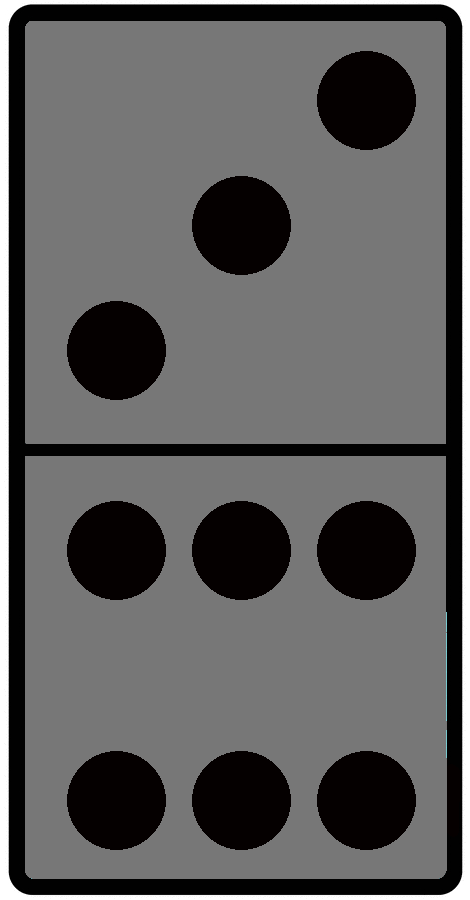
\includegraphics[width=0.05\textwidth]{darkgray3_6v.png}}\ \right]$
\end{center}

That's right: those columns are \textit{blue dominoes.}

\medskip

It turns out that the definition of \textbf{singular} is \textit{a matrix in
which the columns are not linearly independent}. Such a matrix is ``broken'' in
exactly the same way that blue dominoes are broken: its columns don't each
branch out in a brand new direction, and so no matter what linear combination
of them you try to take, you can't reach most points.

If you think about it, that's exactly what we're trying to do here. The above
matrix equation is essentially saying ``find me a linear combination of
${\scriptsize \begin{bmatrix} 2 \\ 4 \end{bmatrix}}$ and ${\scriptsize
\begin{bmatrix} 3 \\ 6 \end{bmatrix}}$ that will land me at the point
${\scriptsize \begin{bmatrix} 8 \\ 11 \end{bmatrix}}$.'' But there is no such
linear combination. I can't take $x$ copies of the first vector and $y$ copies
of the second and get to ${\scriptsize \begin{bmatrix} 8 \\ 11 \end{bmatrix}}$,
because those vectors point in the same dog-gone direction.

\medskip

By the way, it might have occurred to you that it's possible to get extremely
lucky. If we tweak the second of our equations ever so slightly:

\vspace{-.25in}
\begin{align*}
2x + 3y &= 8 \\
4x + 6y &= \textbf{16},
\end{align*}
\vspace{-.25in}

then suddenly it's not only possible to get \textit{a} solution, but
\textit{zillions} of different solutions. All of these work:

\begin{center}
\setlength{\tabcolsep}{13pt}
\renewcommand{\arraystretch}{.8}
\begin{tabular}{cccccc}
$x=1$ & $x=4$ & $x=-2$ & $x=3$ & $x=16$ & \textit{...} \\
\scriptsize and &
\scriptsize and &
\scriptsize and &
\scriptsize and &
\scriptsize and &
\scriptsize and\\
$y=2$ & $y=0$ & $y=4$ & $y=\frac{2}{3}$ & $y=-8$ & \textit{...} \\
\end{tabular}
\end{center}

That's because any pair of numbers that work in the first equation are
automatically going to also work in the second. So it's not quite correct to
say ``a singular matrix means there are no solutions,'' since in very rare
cases it can instead mean ``\textit{too many} solutions.''

\medskip
\pagebreak

\index{injective function}
\index{surjective function}
\index{bijective function}

Lastly, let's complete the connection from section~\ref{sec:functionProps}
(p.~\pageref{sec:functionProps}). You'll recall that if a square matrix is
full-rank, then its linear transformation will be both injective and surjective
(and hence, bijective). Every input vector will be mapped to its \textit{own}
output vector (not sharing that output with any other input vector), and every
possible output vector will have an input that maps to it.

\index{reversible}

This is precisely true for \textit{non-singular} matrices. And here's why: only
non-singular matrices have inverses. A bijective function is reversible: not
only is there a unique output for every input, but there's a unique input for
every output. And so it makes sense that there would be an inverse matrix that
``undoes'' the mapping from input to output. Singular matrices, on the other
hand, do not correspond to bijective transformations at all. Many inputs will
map to the same output, and some outputs won't have any input mapping to them
at all. Thus it's perfectly expected that there be no inverse for such
matrices, because the presence of an inverse implies that we can do the mapping
in both directions.

%\section[The Central Dogma of square matrices]{\large The Central Dogma of square matrices}
\section{The Central Dogma of square matrices}

I've mentioned several times how all of these different ideas are tied
together. Let me now be explicit and complete about that.

\index{yellow matrix}
\index{blue matrix}

Suppose you have a square matrix $A$. There are two possibilities: either its
columns are all linearly independent of each other, or else they aren't. Which
of those two things are true puts $A$ in one of two big categories. I'm going
to call the first type of matrix a ``yellow matrix'' and the second type a
``blue matrix,'' to match our definitions about the linear independence (or
lack thereof) of dominoes.

\pagebreak
The following things are all true for \textbf{yellow} matrices:

\index{linear independence}
\index{inverse}
\index{kernel}
\index{nullity}
\index{full-rank matrix}

\begin{framed}
\begin{compactitem}
\item $A$ is a \textbf{non-singular} square matrix.
\item $A$ has \textit{all linearly independent} columns (yellow dominoes).
\item $A$ is ``full rank.'' (The rank is equal to the dimension of the matrix.)
\item The kernel of $A$ has only the zero vector in it.
\item The nullity of $A$ is 0.
\item $A$ has an \textbf{inverse} matrix, which we can call $A^{-1}$.
\item $A$ represents a system of equations which can be solved (and which has
exactly one solution.)
\item $A$ represents a linear transformation that is bijective.
\end{compactitem}
\end{framed}

\index{singular matrix}

On the flip side, the following are all true for \textbf{blue} matrices:

\begin{framed}
\begin{compactitem}
\item $A$ is a \textbf{singular} square matrix.
\item $A$'s columns are \textit{not} linearly independent (blue dominoes).
\index{rank-deficient}
\item $A$ is ``rank-deficient.'' (The rank is less than the dimension of the
matrix.)
\item The kernel of $A$ has \textit{more} than just the zero vector in it.
\item The nullity of $A$ is greater than 0.
\item There is \textit{no} inverse matrix of A.
\item $A$ represents a system of equations which either can't be solved, or
which has infinitely many solutions.
\item $A$ represents a linear transformation that is neither injective nor
surjective.
\end{compactitem}
\end{framed}

Either all the stuff in the first box is true, or all the stuff in the second
box. There is no in between.
